\section{Learning to Clean Data}
It is widely known that data cleaning is one of the most time-consuming steps of the data analysis process~\cite{nytimes}, and
designing algorithms and systems to automate or partially automate data cleaning continues to be an active area of research~\cite{DBLP:conf/sigmod/ChuIKW16}.
Automation in data cleaning is challenging because real-world data is highly variable. 
A single data set can have many different types of data corruption such as statistical outliers, constraint violations, and duplicates.
Once an error is detected, there is a further question of how to repair this error, which often depends on how the data will be used in the future.

This variability creates a tension between generality and efficiency.
While one might want a single cleaning framework that addresses all types of errors and repair operations, it is far more efficient to consider more specialized frameworks.
Data cleaning tools are often highly optimized for particular problems  (e.g., see statistical outliers~\cite{hellerstein2008quantitative}, enforcing logical constraints~\cite{DBLP:conf/sigmod/ChuIKW16}, entity resolution~\cite{DBLP:journals/pvldb/KopckeTR10}). 
Consequently, a recent survey of industry suggests that data cleaning pipelines are often a patchwork of custom scripts and multiple specialized systems~\cite{krishnan2016hilda}.
The overhead to setup, learn, and manage multiple cleaning systems can easily outweigh the benefits.
Some data scientists eschew automated tools altogether and simply write data cleaning programs from scratch.
The customized programming approach quickly becomes difficult to mantain and interpret; especially for users without data engineering expertise~\cite{sculley2014machine}.

A single cleaning system that exposes a sufficiently flexible interface is clearly desirable; as long as the runtime and accuracy can be made comparable to existing alternatives.  
To achieve this, we turn to the contemporary AI literature, which has produced exciting results such as AlphaGo~\cite{silver2016mastering} that were previously considered not possible.    This work shows that a combination of machine learning and massively parallelized search can effectively optimize highly complex objective functions.
Our main observation is that data cleaning is very similar to the search problems considered in AI~\cite{russell1995modern}.
The classic application is a computer chess program that must plan a sequence of chess moves that change the state of the board in order to maximize the likelihood of a checkmate. Likewise, in data cleaning, one is given a dirty relation and a way to measure data quality (e.g., number of integrity constraints violated), and the data cleaning problem is to find a sequence of modifications to the relation that maximize the data quality metric.

Most non-trivial problems are very hard without good search heuristics.
Advances in machine learning have made it possible to replace hand-crafted heuristics with automatically learned pruning functions that estimate the expected quality of candidate plans. AlphaGo learned pruning heuristics using a neural network trained on data generated through self-play~\cite{silver2016mastering}.
This insight is highly relevant to data cleaning, where datasets tend to have structure amenable to learning heuristics adaptively.
Data errors are often systematic where they are correlated with with certain attributes and values in the dataset~\cite{rekatsinas2017holoclean,DBLP:journals/pvldb/KrishnanWWFG16}.
Consequently, as more data is cleaned, we can better identify common patterns to prioritize the search on future data.
We may not necessarily need a neural network for data cleaning, but the overall algorithmic structure of AlphaGo, tree-search combined with a learned heuristic, can be very useful.

\sys is a new data cleaning system that is designed around a search-based model. It takes as input a {\it quality function} that models the data quality of a relation as a real-value between $[0,1]$ and a {\it language} of parameterized data cleaning operators, and outputs a sequence of data cleaning transformations (a cleaning program) from the language that seeks to maximize the quality function.This API imposes minimal restrictions on the quality function, giving it tremendous flexibility in terms of the data errors that it can express.   As a comparison, a recent system called Holoclean~\cite{rekatsinas2017holoclean} is similar in that it provides a rich interface to specify denial constraints and lookup tables, and integrates them within a probabilistic model to more accurately resolve constraint violations.  In contrast, \sys's quality function is a user-defined function that can express {\it arbitrary combinations} of denial constraints {\it as well as} statistical, quantitative, text formatting, and other classes of data errors.  For instance, \Cref{s:expquant} shows how \sys can perform cleaning for machine learning applications by embedding machine learning training and evaluation within the quality function, while \Cref{s:expterror} combines entity resolution, outlier cleaning, and functional dependency violations within the same function.  


\sys uses a best-first search that greedily appends data transformations to the set of best candidate programs seen so far, and adopts parallelization and pruning ideas from the search-based planning literature.  In contrast to traditional search problems, where the search state (e.g., chess board) is compact and largely trivial to parallelize in a distributed setting, the data cleaning search state is the size of the input dataset and introduces a trade-off between communication costs to share intermediate state and the degree of parallelism possible.  
To further accelerate its runtime, \sys can also encode problem-specific optimizations as search pruning rules (e.g., disallowed transformation sequences) or modifications to the data representation (e.g., clustering similar records).  We find that many optimizations in existing cleaning systems may be cast as search pruning rules.

\sys can adaptively learn pruning rules to avoid unprofitable search branches during the search process.
While AlphaGo used a deep neural network and massive amounts of training data to model the heurisitic, we found that a simple logistic regression classifier and training data gathered during the search process was sufficient to reduce the runtime by multiple orders of magnitude. 
It is important to acknowledge that \sys loses many of the provable guarantees provided by specialized systems based on logical constraints, and is in some sense, best-effort.  
Across 8 real-world datasets used in prior data cleaning literature, we show that \sys matches or exceeds the cleaning accuracy and exhibits competitive run-times to state-of-the-art approaches that are specialized to a specific error domain (constraint, statistical, or quantitative errors).  

\begin{itemize}
\item \stitle{Optimization} Existing cleaning pipelines must combine disparate cleaning solutions and manage glue code to transfer data between systems.  However, data transfer can be a non-trivial portion of the total cleaning cost and recent work~\cite{palkar2017weld} has shown that a common runtime can avoid data movement and improve runtimes by up to $30\times$.  

\item \stitle{Generalization and Robustness} In contrast to existing cleaning systems, that output a cleaning relation, \sys outputs a composable cleaning program that is both simpler to understand because it groups common fixes together, and can be applied to new data.  In addition, the cleaning program allows us to analyze cleaning systems for overfitting.  We indeed find that the complexity of the quality function and cleaning language can lead to overfitting, and believe this is the case for any data cleaning system.  We also show that simple changes to the quality function can act as regularization terms to control the degree of overfitting.

\item \stitle{Software Engineering}  Users do not need to write and manage glue code; do not need to manage ETL between systems; and do not need to learn system specific abstractions, languages, and assumptions.  All of these are arguably intangible, but critical friction points in the highly iterative cleaning process.  

\item \stitle{New Cleaning Applications} We envision that a single API makes it possible to support an ecosystem of domain-specific cleaning specification libraries.  For instance,  interactive visualization interfaces akin to~\cite{trifacta,kandel2011wrangler,DBLP:journals/pvldb/0002M13,wu2012demonstration} can directly translate user interactions into a wide range of cleaning constraints.   
\end{itemize}


\subsection{Problem Setup}
First, we overview the basic formalism of \sys and present its relationship to related work.
We focus on data transformations that concern a single relational table. 
Let $R$ be a relation over a set of attributes $A$,  $\mathcal{R}$ denote the set of all possible relations over $A$, and $r.a$ be the attribute value of $a \in A$ for row $r \in R$.
A data transformation $T(R): \mathcal{R} \mapsto \mathcal{R}$ maps an input relation instance $R \in \mathcal{R}$ to a new (possibly cleaner) instance $R' \in \mathcal{R}$ that is union compatible with $R$.  For instance, ``replace all \texttt{city} attribute values equal to {\it San Francisco} with {\it SF}'' may be one data transformation, while ``delete the $10^{th}$ record'' may be another.   
Aside from union compatibility, transformations are simply UDFs.
Although it is desirable for the transformation to be deterministic and idempotent, if they are not, it simply makes the cleaning problem harder.
%We find that nearly all cleaning transformations in existing literature satisfy these properties \ewu{(See Appendix of technical report)}. 

Data transformations can be composed using the binary operator $\circ$ as follows: $(T_i \circ T_j)(R) =  T_i(T_j(R))$.
The composition of one or more data transformations is called a {\it cleaning program} $p$.   If $p = p' \circ T$, then $p'$ is the parent of $p$; the parent of a single data transformation is a NOOP.  In practice, users will specify {\it transformation templates} $\mathbb{T}(\theta_1,\cdots,\theta_k)$, and every assignment of the parameters represents one possible transformation.  
Although $\mathbb{T}$ can in theory be an arbitrary deterministic template function, our current implementation makes several simplifying assumptions to bound the number of data transformations that it can output.  We assume that a parameter $\theta_i$ is typed as an attribute or a value.  The former means that $\theta_i$'s domain is the set of attribute names in the relation schema; the latter means that $\theta_i$'s domain is the set of cell values found in the relation, or otherwise provided by the user. 

\begin{example}\label{ex1}
The following \texttt{City} relation contains two attributes \textsf{city\_name} and \textsf{city\_code}.  Suppose there is a one-to-one relationship between the two attributes. In this case, the relation is inconsistent with respect to the relationship and contains errors highlighted in \red{red}.

  \begin{table}[ht!]
	\small
  \centering
  \label{my-label}
  \begin{tabular}{|l|l|l|}
  \hline
  \rowcolor[HTML]{000000} 
  & \white{city\_name}            & \white{city\_code}   \\ \hline
  1 & San Francisco                    & SF                                  \\ \hline
  2& \red{\textbf{New York}}           & NY                                  \\ \hline
  3 & New York City                    & \red{\textbf{NYC}} \\ \hline
  4 & \red{\textbf{San Francisc}}      & SF                                  \\ \hline
  5 & San Jose                         & SJ                                  \\ \hline
  6 & San Mateo                        & SM                                  \\ \hline
  7 & New York City                    & NY                                  \\ \hline
  \end{tabular}
  \end{table}

The following transformation template uses three parameters: \texttt{attr} specifies an attribute, \texttt{srcstr} specifies a source string, and \texttt{targetstr} specifies a target string.   
{\small\[
T = \textsf{find\_replace}(\text{srcstr}, \text{targetstr}, \text{attr})
\]}
The output of the above is a transformation $T$ that finds all \texttt{attr} values equal to \texttt{srcstr} and replaces those cells with \texttt{targetstr}. 
For instance, \texttt{find\_replace(``NYC'', ``NY'', ``city\_code'')(City)} returns a data transformation that finds records in \texttt{City} whose city\_code is ``NYC'' and replaces their value with ``NY''.
\end{example}


Let $\Sigma$ be a set of distinct data transformations $\{T_1,\cdots,T_N\}$, and
$\Sigma^*$ be the set of all finite compositions of $\Sigma$, i.e., $T_i\circ T_j$.
A formal language $L$ over $\Sigma$ is a subset of $\Sigma^*$.
A program $p$ is valid if it is an element of $L$.

\begin{example}\label{ex2}
  Continuing \Cref{ex1}, $\Sigma$ is defined as all possible parameterizations of \texttt{find\_replace}.  Since many possible possible parameterizations are non-sensical (e.g., the source string does not exist in the relation), we may bound $\Sigma$ to only source and target strings present in each attribute's instance domain (a standard assumption in other work as well~\cite{DBLP:series/synthesis/2012Fan}).  In this case, there are $61$ possible data transformations, and $\Sigma^*$ defines any finite composition of these $61$ transformations.  The language $L$ can be further restricted to compositions of up to $k$ data transformations.  
\end{example}

Finally, let $Q(R): \mathcal{R} \mapsto [0,1]$ be a quality function where $1$ implies that the instance $R$ is clean, and a lower value correspond to a dirtier table.
Since running a program $p\in\mathcal{L}$ on the initial dirty table $R_{dirty}$ returns another table, $Q(p(R_{dirty}))$ returns a quality score for each program in the language.  
$Q$ is a UDF and we do not impose any restrictions on it. In fact, one experiment embeds training and evaluating a machine learning model {\it within} the quality function (\Cref{s:expquant}).  Another experiment shows that \sys can be robust to random noise injected in the function (\Cref{s:expoverfit}).   

Even so, we call out two special cases that provide optimization opportunities. 
We define two sub-classes of quality functions: row-separable and cell-separable quality functions.
The former expresses the overall quality based on row-wise quality function $q(r): R \mapsto [0,1]$ where $0$ implies that the record is clean:
$Q(R) \propto \sum\nolimits_{r \in R} q(r)$
Similarly, a cell-separable quality function means that there exists a cell-wise quality function $q(r, a): (R\times A) \mapsto [0,1]$, such that the quality function is the sum of each cell's quality: 
$Q(R) \propto \sum\nolimits_{r \in R} \sum_{a \in A} q(r,a)$.

These special cases are important because they can define hints on what types of transformations are irrelevant.
For example, if the quality function is cell-separable, and we have identified that a set of cells $C$ are dirty (e.g., they violate constraints), then we can ignore transformations that do not modify cells in $C$.  This restricts the size the language and makes the problem much easier to solve.


\noindent We are now ready to present data cleaning as the following optimization problem:
\begin{problem}[$\textsf{clean}(Q,R_{dirty},L)$]
Given quality function $Q$, relation $R_{dirty}$, and language $L$, find valid program $p^* \in L$ that optimizes $Q$:
\[
p^* = ~ \min_{p \in L} Q( p(R_{dirty}) ).  
\]
\end{problem}
$p^*(R_{dirty})$ returns the cleaned table, and $p^*$ can be applied to any table that is union compatible with $R_{dirty}$.
A desirable property of this problem formulation is that it directly trades off runtime with cleaning accuracy and can be stopped at any time (though the cleaning program may be suboptimal).  At the limit, \sys simply explores $L$ and identifies the optimal program.


\begin{example}\label{ex3}
Continuing~\Cref{ex1}, let us assume the following functional dependencies over the example relation: $\textsf{city\_name} \rightarrow \textsf{city\_code}$ and $\textsf{city\_code} \rightarrow \textsf{city\_name}$.
We can efficiently identify inconsistencies by finding the cities that map to $>1$ city code, and vice versa.   Let such city names and codes be denoted $D_{city\_name}$ and $D_{city\_code}$, respectively.
$Q(R)$ is a cell-separable quality function where the cell-wise quality function is defined as $q(r, a) = 1 - (r.a \in D_a)$, such that $r.a$ is $1$ if the attribute value does not violate a functional dependency, and $0$ otherwise.

By searching through all possible programs up to length 3 in $L$, we can find a cleaning program based on \texttt{find\_replace} that resolves all inconsistencies:
\begin{lstlisting}
    find_replace(New York, New York City, city_name)
    find_replace(San Francisc, San Francisco, city_name)
    find_replace(NYC, NY, city_code)
\end{lstlisting}
\end{example}


\subsubsection{Approach Overview and Challenges}
Our problem formulation is a direct instance of {\it planning} in AI~\cite{russell1995modern}, where an agent identifies a sequence of actions to achieve a goal.  In our setting, the agent (\sys) explores a state space ($\mathcal{R}$) from an initial state (the input relation) by following transitions (applying $T_i \in \Sigma$) such that the sequence of actions is valid (within $\Sigma^*$) and the quality of the final state ($Q(R_{final})$) is maximized.  

For readers familiar with stochastic processes, this search problem is equivalent to a deterministic Markov Decision Process (MDP), where the states are $\mathcal{R}$, the actions $\Sigma$, the transition function updates the instance with the transformation, the initial state is the dirty instance $R_{dirty}$, and the reward function is $Q$.

One may be hesitant in adopting our problem formulation because, although it is sufficiently general to model many existing data cleaning problems, such generality often comes at the expense of runtime performance.   The planning problem is APX-Hard, meaning there does not exist a polynomial time approximation unless P=NP.  
Let $R$ be a single-attribute relation of Booleans. Let $L$ be the set of all assignments to a single value.
Given a list of $N$ Boolean clauses over all the boolean variables, let $Q$ assign to each record one minus the fraction of clauses that evaluate to true. This formulation is equivalent to MAX-SAT and solution to the optimization problem. 

For this reason, {\it the key technical challenge is to show that \sys can solve data cleaning problems with comparable run-time as existing specialized systems, and can be easily extended to support new optimizations.}
Despite the problem's worst-case complexity, 
recent successes in similar planning problems---ranging from AlphaGo~\cite{silver2016mastering} to automatically playing Atari video games~\cite{mnih2015human} have shown that a prudent combination Machine Learning and distributed search can find practical solutions by leveraging the structure of the problem. 
Not every problem instance is as pathological as the worst case complexity suggests, and there are many reasonable local optima.


\subsection{Architecture and API}
\begin{figure}[t]
% \vspace{-5pt}
\centering
 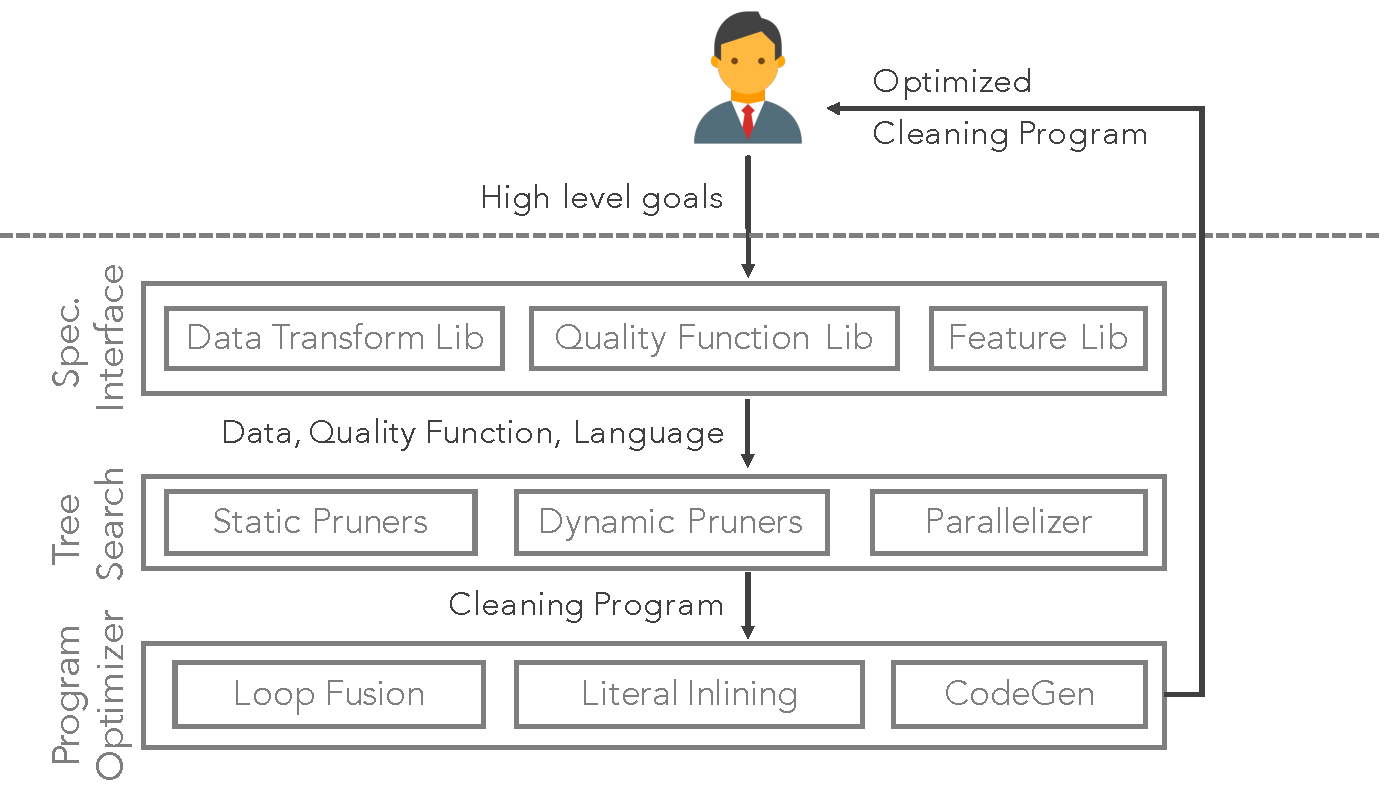
\includegraphics[width=.8\columnwidth]{ac-experiments/alphacleanarch.pdf}
 \caption{\small \sys transforms high level cleaning goals (e.g., integrity constraints, statistical models, cleaning operations) into a quality measure and cleaning language, and uses an optimized tree search to find and optimize a sequence of transformations (cleaning program) to maximize the quality measure.   \label{fig:arch} }
\end{figure}
This section describes the three major components of the \sys system architecture (\Cref{fig:arch}), split between the user interface to specify the cleaning problem, the core search algorithm, and optimization of the resulting cleaning program.  We detail the interface and program optimization in this section, and focus on the search algorithm and optimizations in the rest of the paper. Designing data cleaning interfaces~\cite{DBLP:conf/uist/GuoKHH11} and query optimization for data cleaning~\cite{DBLP:conf/vldb/GalhardasFSSS01, khayyat2015bigdansing} are interesting problems in their own right, and we believe \sys can enable simpler and more powerful approaches.  However, these were not a focus of the current study.

The {\it Specification Interface} contains extensible libraries of domain-specific quality functions, cleaning data transformations, and pruning feature hints that the user can use to define a high level cleaning goal.  Our current implementation can translate a wide range of domain-specific goals---including type constraints, functional dependencies, denial constraints, lookup tables, parametric and non-parametric outlier models, and correlations between numeric attributes---into a single quality function.  Users can also constrain the cleaning language, and we currently support any type of conditional cell and record transformation that applies a black-box transformation to all cells or records satisfying a predicate; both the transformation parameters and the predicate are learned by \sys.  Finally, users can optionally provide features that \sys uses to dynamically learn pruning rules (Section~\ref{s:dynlearn}).

The {\it Search} component takes as input the quality function $Q$ and language $L$, and performs a greedy search heuristic to find a program $p^* \in L$ that maximizes $Q$.  Users can supply hints that exploit the problem structure to reduce the runtime by pruning the search space and parallelizing the search.  To bound the search space, users specify a maximum program length $k$.    \sys also supports three classes optimizations. {\it Static pruning} invalidates candidate programs based on the program structure (sequence of actions).  For instance, composing the same idempotent transformation (e.g., \texttt{find\_replace(SFO, SF, city\_name)}) in succession is unnecessary.  {\it Dynamic pruning} can access the result of a candidate program (search state) when making pruning decisions, and we propose a novel approach to learn automatic dynamic pruning rules that can reduce end-to-end runtimes by up to 75\% at the expense of slightly lower recall. Finally, \sys ~ {\it parallelizes} ~ the search in both shared memory and distributed settings.  Section~\ref{s:opts} describes the pruning rules and parallelization optimization in detail.


Finally, once search component outputs the cleaning program $p^*$, the {\it Program Optimizer} performs query compilation optimizations and provides an API to add new optimizations.  \sys currently replaces variables with literal values whenever possible, inlines data transformations into loops that scan over the input relation, and uses loop fusion~\cite{palkar2017weld, crotty2014tupleware} to avoid unnecessary scans over the input and intermediate relations for each transformation in $p^*$.  Consider the program in~\Cref{ex3}.  Since the \texttt{find\_replace} operations do not conflict, it is inefficient to loop through over the relation instance three separate times.  Since they do not conflict, it would be inefficient to execute them sequentially and iterate over the data three separate times.  Instead, they can be fused:
{\small
\begin{lstlisting}
    for r in rows:
     if r[city_name] == `New York':
       r[city_name] = `New York City'
     elif r[city_name] == `San Francisc':
       r[city_name] = `San Francisco'
     if r[city_code] == `NYC'
       r[city_code] = `NY'
\end{lstlisting}
}
These simple optimizations improve the final program runtime by up-to 20x, and we leave further improvements to future work (e.g., could be optimized with a framework like Weld~\cite{palkar2017weld}).


\subsection{Search Algorithm}
We now provide an overview of \sys's search algorithm and optimizations.

% The optimization algorithm takes a quality function, a language, and a dirty relation, and outputs a sequence of transformations (of max depth $k$) that maximizes the quality function.

{
\begin{algorithm}[t]
\KwData{Q, R, $\Sigma$, $L$, (k, $\gamma$)}

// Initialize priority queue of candidate programs\\
$P = \{NOOP\}$

\While{ $|\{p \in P\ |\ p.len < k\}| > 0$ }
{
    \For{$p \in P: \|p\| < k$ }{
        
        Pop $p$ from the queue.
        
        \For{$T \in \Sigma$}{
             $p' = p \circ T$ 
             
             \If{$p' \in L$}{
               $P.push(p', Q(p'(R)))$
             }
        }
    }
    
    $\bar{p} = \argmax_{p\in P} Q(p(R))$\\
    $P = \{p \in P\ |\ p < \gamma\times Q(\bar{p}(R)) \}$
}

\Return Highest priority item on the queue
\caption{Greedy Best-First Tree Search}
\label{alg:main}
\end{algorithm}
}

\subsubsection{Naive Search Procedures}
In principle, any tree search algorithm over $L$ would be correct.
However, the traversal order and expansion policy is important in this search problem.  We describe the algorithmic and practical reasons why two naive procedures---breadth-first search (BFS) and depth-first search (DFS)---exhibit poor search runtimes.

\stitle{BFS} This approach extends each program in the search frontier with every possible data transformation in $\Sigma$.  To extend a candidate program $l_c$ with $T \in \Sigma$, it evaluates $Q((T\circ l_c)(R))$.  Unfortunately, the frontier grows exponentially with each iteration.  Additionally, evaluating every new candidate program $T\circ l_c$ can be expensive if the input relation is large.   Although the cost can be reduced by materializing $l_c(R)$, it is not possible to materialize all candidate programs in the frontier for all but the most trivial cleaning problems.    It is desirable to use asearch procedure that bounds the size of the frontier and the materialization costs.

 The first problem with this algorithm is that since each node in this tree $o$ represents a sequence of transformations.
 Evaluating the value of $o$ can be very expensive since it would have to evaluate the entire path to the root.
 $o$ is a composition of many transformations and may require a number of passes over the dataset.
 This can be avoided if we can materialize (either to disk or memory) the frontier,that is, for each node in the priority queue $o \in O$, we have a cached result of $o(R)$. 
 However, with BFS, the frontier is exponential in the support of the language and the system would quickly run out of memory.

\stitle{DFS} Depth-first search only needs to materialize the intermediate results for a single program at a time, however it is highly inefficient since the vast majority of programs that it explores will have low quality scores.  


\subsubsection{Search Algorithm and Optimizations}
Best-first search expands the most promising nodes chosen according to a specified cost function.
We consider a greedy version of this algorithm, which removes nodes on the frontier that are more than $\gamma$ times worse than the current best solution (\Cref{alg:main}).
Making $\gamma$ smaller makes the algorithm asympotically consistent but uses more memory to store the frontier, whereas $\gamma=1$ is a pure greedy search with minimal memory requirements.  

The frontier is modeled as a priority queue $P$ where the priority is the quality of the candidate program, and is initialized with a NOOP program with quality $Q(R)$.  
The algorithm iteratively extends all programs in the queue with less than $k$ transformations; a program $p$ is extended by composing it with a transformation $T$ in $\Sigma$.  If the resulting program $p'$ is in the language $L$, then we add it to the queue.
Finally, let $\bar{p}$ be the highest quality program in the queue.  The algorithm removes all programs whose quality is $<\gamma\times Q(\bar{p}(R))$ from the frontier.  
This process repeats until the candidate programs cannot be improved, or all programs have $k$ transformations.

In a naive and slow implementation, the above algorithm computes $p$'s quality by fully running $p$ on the input relation before running $Q$ on the result, explores all possible data transformation sequences, and runs sequentially.  One of the benefits of its simple structure is that it is amenable to a rich set of optimizations to prune the search space, incrementally compute quality functions, and parallelize the search.  In fact, we find that many optimizations in existing specialized cleaning systems can be cast in terms of the following classes.

 We can materialize (either to disk or memory) the frontier,that is, for each node in the priority queue $p \in P$, we have a cached result of $p(R)$. 
 Then, when we expand the nodes to $p' = p \circ t$, we only have to incrementally evaluate $t(R)$.
 After the node is expanded, the result is added to the cache if it within $\gamma$ of the best solution.
 The basic algorithm described above is well-suited for this problem.
 Without the greediness, the frontier might be exponentially large leading to an impractical amount of materialization.
 By tuning $\gamma$, the user can essentially set how much memory is used for materialization.


\btitle{Static Pruning Rules} are boolean functions that take a candidate program $p$ as input and decides whether it should be pruned. \sys currently models static rules as regular expressions over $\Sigma$.  Static rules are can be viewed as filters over $L$.
\[\textsf{static\_rule}(p) \mapsto \{0,1\}\]
For example, since the find-and-replace operations are idempotent, i.e., $T(T(R)) = T(R)$, we may want to only consider the set of all sequences with no neighboring repeated transformations. Similarly, we may also want to prune all search branches that make no effect (i.e., find-and-replace New York with New York).
These two regular expressions alone reduce the above example's language by $48\%$ (from 226981 to 120050).
Other rules, such as avoiding changes that undo previous changes $T^{-1}(T(R)) = R$, are similarly easy to add.


\btitle{Dynamic Pruning Rules} also have access to the input relation and quality function, and can make instance-specific pruning decisions.
\[\textsf{dyn\_rule}(p, Q, R) \mapsto \{0,1\}\]
For example, suppose  $Q$ is based on functional dependencies and is cell-separable, and we want to ensure that cell-level transformations made by a candidate program $p$ individually improve $Q$.  In this case, we find the cells $C$ that initially violate the functional dependencies and ensure that the cells transformed by $p$ are all in $C$.  Applying this optimization, in addition to the others in \sys, to the example reduces the search space by $143\times$ from 226,981 candidate programs to only 1582.  

Since it can be challenging to hand-write pruning rules, \Cref{s:dynlearn} describes a dynamic approach that uses simple machine learning models to automatically identify the characteristics of candidate programs to decide whether a particular search brach will be promising.  In essence, it generates and refines static pruning rules during the search process.  

%  it is a promising  and relation instance to decide whether the candidate program is promising to further explore.  In essense, it estimates the quality function of the search space rooted at $p$.

For example, we may want to ensure that all the evaluations are ``correlated'' with the cost function--that is it makes modifications that are likely to affect the costs.  This is possible if the cost separable where we have a score for each cell. In this case, we can find all the cells in violation of the functional dependencies and make sure that the ``source'' field of the find-and-replace operations only match values that are in violation.  These optimizations are called ``dynamic' because they can be determined from the active domain (i.e., after applying a transformation, recalculate new optimization rules).  Applying this optimization (in addition to the others) to the example reduces the search space to 1582 evaluations v.s. 226981 unoptimized (143x reduction).

\stitle{Block-wise Cleaning} 
A major cost is that independent errors in the relation must be cleaned sequentially in the search algorithm.  For instance, records 2, 3, and 4 in~\Cref{ex1} exhibit independent errors and a fix for a given record does not affect the other records.  Thus, if each record were cleaned in isolation, the search space would be $O(|\Sigma|)$.  Unfortunately, the entire relation requires a program of three transformation to fix the records, which increases the search space to $O(|\Sigma|^3)$.

The main insight in block-wise cleaning is that many errors are local to a small number of records.  In these cases, it is possible to partition $R$ into a set of blocks $B_1,\cdots,B_m$, execute the search algorithm over each block independently, and concatenate their programs to generate the final cleaning program.  This gather-scatter approach can exponentially reduce the search space for each block, and reduces the cost of evaluating super-linear quality functions that require e.g., computing a pair-wise similarity scores for the input relation.    For example, quality functions derived from functional dependencies can define blocks by examining the violating tuples linked through the dependency.  Similarly, users can define custom partitioning functions or learn them via e.g., clustering algorithms.  In our current implementation, we partition the input relation by cell or row if the quality function is cell or row separable.


\stitle{Parallel Program Evaluation} It is clear that the candidate programs can be evaluated and pruning in a parallel fashion across multiple cores and multiple machines, and is one of the major innovations in modern planning systems.  However, unlike classic planning problems where communications are small due to the compact size of each state, \sys's state size is determined by the relation instance, and can lead to prohibitively high communication costs and memory caching requirements.   Section~\ref{s:parallel} describes how we manage the trade-offs when parallelizing \sys in shared memory and distributed settings.

\stitle{Materialization} Since each candidate program $p' = p\circ T$ is the composition of a previous candidate program and a transformation, an obvious optimization is to materialize the output of $p(R)$ and incrementally compute $p'(R)$ as $T(p(R))$ over the materialized intermediate relation.  Although this works well in a single threaded setting, memory and communication challenges arise when combining materialization with parallelization (\Cref{s:parallel}).



\subsection{Experiments}\label{s:exp}
Next, we present experimental results that suggest three main conclusions: (1) as a single framework, \sys can achieve parity in terms of accuracy with state-of-the-art approaches to a variety of different problems ranging from integrity constraint satisfaction, statistical data cleaning, and also data cleaning for machine learning, (2) it is possible to significantly reduce the runtime gap between \sys and specialized frameworks using simple pruning and distributed parallelization techniques, and (3) \sys enables automatic data cleaning for datasets containing a mixture of error types in an acceptable amount of time.  

\subsubsection{Datasets and Cleaning Tasks}
We list the main characteristics of the 8 experimental datasets.

\stitle{Flight} The flight dataset~\cite{data-flights} contains arrival time, departure time, and gate information aggregated from 3 airline websites (AA, UA, Continental), 8 airport websites (e.g., SFO, DEN), and 27 third-party websites.
There are 1200 flight departures and arrivals at airline hubs recorded from each source.  Each flight has a unique and globally consistent ID, and the task is to reconcile data from different sources using the functional dependency \texttt{ID$\rightarrow$ arrival, departure, gate information}.

% The data cleaning problem is to reconcile the differences between each sources.  Each flight has a unique flight identifier that is consistent across the websites.  Formally, we can model the reconciliation problem as functional dependency between the flight id and the arrival time, departure time, gate information.  This enforces that after resolution there will be a single canonical version of those values.

\stitle{FEC} The election contributions dataset has 6,410,678 records, and 18 numerical, discrete, and text attributes. This dataset records the contribution amount and contributor demographic information e.g., name, address, and occupation.  The task is to enforce \texttt{city$\rightarrow$zipcode}, and match occupation to a codebook on canonical occupations.  The quality function is 1 if the occupation is in the codebook, and 0 otherwise; we penalize the edit distance between the original and edited occupation values.

% In this dataset, we enforced functional dependency relationships between city and zipcodes. We also matched the occupation of the contributors to a code book of popular occupations. This was posed as a quality function that was 1 only if the cell belonged to the code book and 0 otherwise, and there was an additive penalty on the edit distance between the change and the previous value.   


\stitle{Malasakit} This dataset contains 1493 survey disaster preparedness responses from the Philippines, with 15 numeric and discrete attributes. The task removes improper numerical values and remove dummy test records. This consists of domain integrity constraints that force the values to be within a certain dictionary.

\stitle{Physician} This dataset from Medicare.gov contains 37k US physican records, 10 attributes, with spelling errors in city names, zipcodes, and other text attributes. We use the data cleaning rules described in~\cite{rekatsinas2017holoclean}, which consists of 9 functional dependencies. 

\stitle{Census} This US adult census data contains 32k records, and 15 numeric and discrete attributes.  There are many missing values coded as 999999.  The task is to clean numeric values to build a classification model that predicts whether an adult earns more than $\$50k$ annually. 

\stitle{EEG}  The 2406 records are each a variable-length time-series of EEG readings (16 numeric attributes), and labeled as ``Preictal'' for pre-seizure and ``Interictal'' for non-seizure.  The goal is to predict seizures based on 32 features computed as the mean and avriance of the numeric EEG attributes.  The task is to identify and remove outlier reading values.  

% The training data is organized into ten minute EEG clips labeled "Preictal" for pre-seizure data segments, or "Interictal" for non-seizure data segments.  There are 2406 records each of which is a variable-length time-series of 16 attributes. We featurize this dataset into records of 32 attributes--the mean and variance over the length of the time-series.  This dataset primarily contains numerical outliers, the clips have spurious readings.

\stitle{Stock} There are 1000 ticker symbols from 55 sources for every trading day in a month~\cite{data-flights}.  The cleaning task involves (1) integrating the schemas by matching attributes across the sources (e.g., `prev. close' vs `Previous Close'), and then (2) reconciling daily ticker values values using primary-key-based functional dependencies akin to the flight dataset.

\stitle{Terrorism} The Global Terrorism Database~\cite{data-terrorism} is a dataset of around terrorist attacks scraped from news sources.  Each record contains the date, location, details about the attack, and the number of fatalities and injuries.  The dataset contains a mixture of data errors:
(1) there are many duplicates for the same terrorist incident,
(2) many missing values in the fatalities and injuries attributes are encoded as zeros, which overlaps with attacks that did not have any fatalities/injuries, and
(3) the location attributes are inconsistently encoded.  
We used the dataset from 1970, and there are $170000$ records.  
We downloaded this dataset and sought to understand whether terrorist attacks have become more lethal than they were in the 1970s.  To do so, we hand cleaned the records to create a gold standard.  It turns out that, in this dataset, attacks have become more lethal, but fewer in number than 50 years ago.  This task was intentionally open-ended to represent the nature of the iterative analysis process.



\begin{figure}
    \centering
    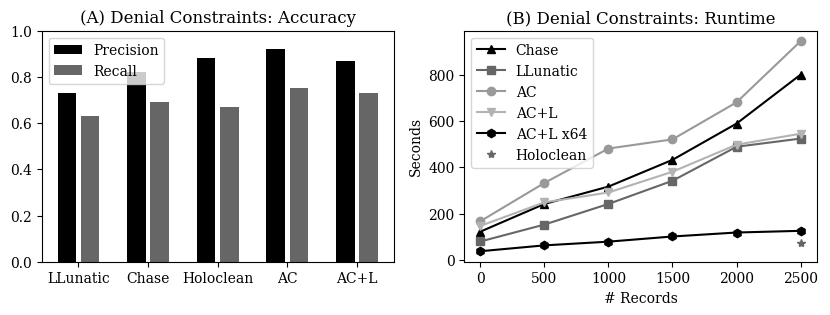
\includegraphics[width=\columnwidth]{ac-experiments/exp1.png}
    \caption{\small Comparison with denial constraint systems on the Flight dataset.  (A) \sys (AC) matches or exceeds the accuracy of the specialized systems.  (B) The structure of the data errors, along the learning and parallelization (AC+L x64) lets \sys scale sub-linearly and outperform all but HoloClean's reported runtimes.  \label{exp1a}}
\end{figure}

\subsubsection{Denial Constraints}
Denial constraints express a wide range of integrity constraints and form the basis of many data cleaning systems.  Although \sys may not fully enforce integrity constraints, we can compose a quality function can quantifies the number of constraint violations and find transformation that reduce the number of violations.    We use the Flight dataset for these experiments.

% Several data cleaning systems use Denial Constraints for constraint specification.  While \sys does not enforce integrity constraints, we can create a data quality objective function that quantifies the number of unsatisfied constraints.  This will search over a set of transformations that maximally satisfy these constraints.

\stitle{Baselines} We run against (1) Llunatic, a denial constraint-based cleaning system~\cite{DBLP:conf/sigmod/DallachiesaEEEIOT13} implemented in C++ on top of PostgreSQL\footnote{Constraints are specified as Tuple-Generating Dependencies}, and (2) a restricted chase algorithm~\cite{benedikt2017benchmarking} implemented in Python. We compare against the chase because a large portion of denial constraints are functional dependencies, and can be resolved using fixed-point iteration.  We report numbers from the recent Holoclean publication~\cite{rekatsinas2017holoclean} that used the same datasets and constraints, but did not run the experiment ourselves.

\stitle{Results} Figure \ref{exp1a}a shows the precision and recall of each approaches based on known ground truth. \sys matches or beats the accuracy of the baselines, however its runtime (AC) without any learning scales poorly compared to alternatives (Figure~ \ref{exp1a}b).  Using learning (AC+L) shows performance on par with LLunatic, and parallelization on 64 threads is comparable to Holoclean's reported runtime. The results suggest that learning exhibits sublinear scaling due to \sys learning more effective pruning rules as it sees more data.  These performance gains are at the expense of slightly reduced accuracy. 

We also evaluated \sys (single threaded, without learning) on the FEC, Malasakit, and Physician datasets.  Their precision, recall, and runtimes are as follows: 
FEC: $94\%$ prec, $68\%$ rec, $5$hrs; 
Malasakit: $100\%$ prec, $85\%$ rec, $0.39$hrs;
Physician: $100\%$ prec, $84\%$, $3.4$hrs.

% \begin{table}[ht]
% \footnotesize
% \small
% \centering
% \begin{tabular}{|l|r|r|r|r|r|r|r|}
% \hline
%  & \#rows & \#cols & Precision & Recall & Runtime \\
% \hline
% \hline
% FEC	&6M&18&0.94&	0.68&	5hrs\\
% \hline
% Malasakit &1493& 15& 1.0 & 0.85& 0.39hrs\\
% \hline
% Physican	&37k&10&1.0&0.84& 3.2hrs\\
% \hline
% \end{tabular}
% \end{table}

\begin{figure}
    \centering
    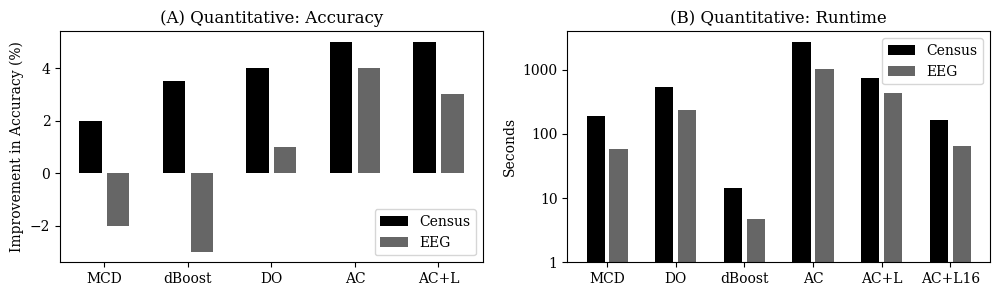
\includegraphics[width=\columnwidth]{ac-experiments/exp2.png}
    \caption{\small Quantitative data cleaning on census and EEG datasets for a classification application.  \sys tranformation can clip outliers or set them to a default value. (A) \sys ha higher accuracy than outlier detection algorithms (MCD, dBoost), and \sys with a single transform template (DO).  (B) Optimizations improve \sys runtime by over an order of magnitude.  \label{exp2a}}
\end{figure}

\subsubsection{Quantitative Data Cleaning}\label{s:expquant}
This experiment performs numerical cleaning on machine learning data.  In these applications, prediction labels and test records are typically clean and available (e.g., results of a sales lead), whereas the training features are often integrated from disparate sources and exhibit considerable noise (e.g., outliers).  Our quality function is simply defined as the model's accuracy on a training hold-out set, and we report the test accuracy on a separate test set.

We trained a binary classification random forest model using \texttt{sklearn} on the Census and EEG datasets.  We used standard featurizers (hot-one encoding for categorical data, bag-of-words for string data, numerical data as is) similar to~\cite{gokhale2014corleone}. 
We split the dataset into 20\% test and 80\% training, and further split training into 20/80 into hold-out and training.  We run the search over the training data, and evaluate the quality function using the hold-out.  Final numbers are reported using the test data.


% The quality function for \sys is 0 for each record that is incorrectly predicted by the model, 1 for each record that is correctly predicted by the model.


% In many machine learning settings, cleanly labeled test data is often available (e.g., the results of following a sales lead). 
% Labels often represent directly observed phenomena making them relatively clean, while features are often weaker signals integrated from multiple disparate sources and subject to error and frequent change.
% This allows us to define a quality function in terms of the model's predictive accuracy--the data cleaning being a means to improving that predictive accuracy.

We defined the following three data transformation templates that sets numerical attribute values in $R$ if they satsify a predicate:

{\small
\begin{itemize}[leftmargin=*, topsep=0mm, itemsep=0mm]
  \item \stitle{\textsf{clip\_gt(attr, thresh)}} $R.attr = thresh$ if $R.attr>thresh$
  \item \stitle{\textsf{clip\_lt(attr, thresh)}} $R.attr = thresh$ if $R.attr<thresh$
  \item \stitle{\textsf{default(attr, badval)}} $R.attr$ set to mean val if $R.attr=badval$
\end{itemize}
}

\stitle{Baselines} We compare with 4 baselines: {\it No Cleaning (NC)}, {\it Minimum Covariance Determinant (MCD)} is a robust outlier detection algorithm used in~\cite{bailis2016macrobase} and sets all detected outliers to the mean value, {\it dBoost} uses a fast partitioned histogram technique to detect outliers~\cite{mariet2016outlier}, and {\it Default Only (DO)} runs \sys with only the \textsf{default()} transformation.  

\stitle{Results} The classifer achieves 82\% and 79\% accuracy on the uncleaned census and EEG data, respectively.  Most outliers in the census data are far from the mean, so MCD and dBoost can effectively find.  Further, setting census outliers to the mean is sensible. However, the same fix is not appropriate for the EEG data; it is better to clip the outlier values, thus MCD, dBoost, and DO have negligible or negative impact on accuracy.  When we realized this from running DO, it was straightforward to add the clipping transformations to the language, and with no other changes, re-run \sys with drastically improved EEG accuracies.  

Vanilla \sys (AC) is nearly $10\times$ slower than MCD, but the adding learning and 16-thread parallelization  matches MCD's runtimes.  dBoost is specialized for fast outlier detection and \sys is unlikely to match its runtime.  


\begin{figure}
    \centering
    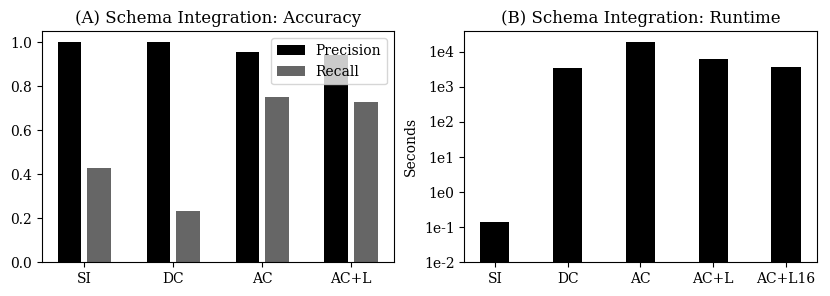
\includegraphics[width=\columnwidth]{ac-experiments/exp3.png}
    \caption{\small Schema integration and functional dependency errors in the stock dataset.  Cleaning schema integration (SI) or functional dependencies (DC) in isolation results in high precision but poor recall.  \sys cleans both types of errors with higher recall, and is as fast as DC.  \label{exp3a}}
\end{figure}

\begin{figure}[ht]
    \centering
    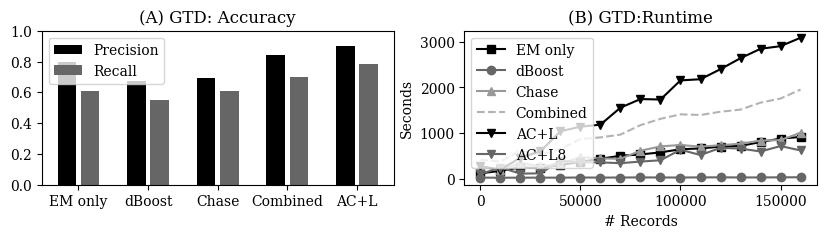
\includegraphics[width=\columnwidth]{ac-experiments/exp7.png}
    \caption{The Global Terrorism Database is a dataset of terrorist attacks scraped from news sources since 1970. (A) Shows that \sys can integrate many different forms of cleaning that were previously handled by disparate systems, (B) \sys achieves a competitive runtime to using all of the different system and accounting for data transfer time between them. \label{exp7a}}
\end{figure}

\subsubsection{Schema Integration}
We now evaluate cleaning on the stock dataset~\cite{data-flights} from 55 different sources that contains a mixture of schema integration and functional dependency errors.

\vspace{0.5em}\noindent\textbf{Baselines: } We compare approaches for each error type in isolation.  Schema Integration  (SI) matches attributes based on attribute name string similarity, and Data Cleaning (DC) assumes schemas are consistent and enforces functions dependencies using a restricted chase~\cite{benedikt2017benchmarking}.

\vspace{0.5em}\noindent\textbf{Results: } The specialized cleaning approaches exhibit high precision but low recall, as they miss records with multiple errors (\Cref{exp3a}).  \sys can mix both tasks in the quality function and has comparable precision with much higher recall.  SI is significantly faster since it only reads schema metadata, however \sys with learning and 16 threads is competitive with DC.

\begin{figure}[ht]
    \centering
    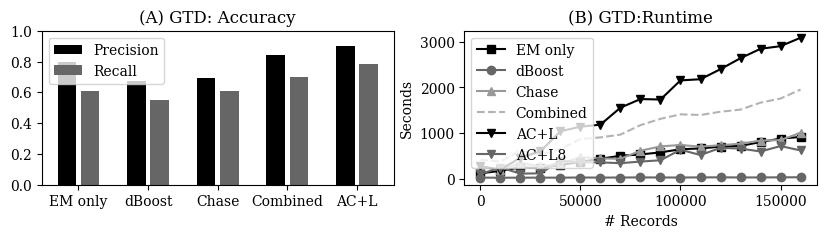
\includegraphics[width=\columnwidth]{ac-experiments/exp7.png}
    \caption{\small The terrorism dataset contains 3 classe of errors. (A) A unified cleaning framework outperforms individual cleaning approaches and even a serial combination.  (B) \sys is easily parallelized to 8 threads to outperform the combined baselines.  \label{exp7a}}
\end{figure}

\begin{figure*}[ht]
\centering
 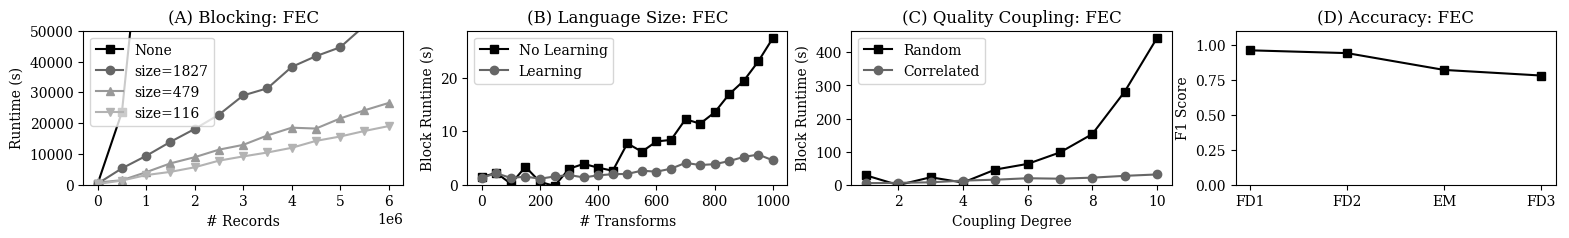
\includegraphics[width=\textwidth]{ac-experiments/exp4.png}
 \caption{\small (A) The degree of block-wise partitioning directly affects search time, (B) increasing the transformation language $\Sigma$ exponentially increases the search time, but learning is very effective at pruning the increased search space, (C) quality functions that couple errors between random records are significantly harder to optimize, (D) \sys degrades gracefully when adding irrelevant error types to the problem.  
 \label{fig:microbenchmarks}}
\end{figure*}

\subsubsection{Mixing Error Classes}\label{s:expterror}
This experiment, we use the multi-error Terrorism dataset~\cite{data-terrorism}. 

\stitle{Baselines} We hand-coded blocking-based entity matching (EM)  and restricted chase (FD) algorithms in Python, and used dBoost for missing values.  We also ran EM, dBoost, and Chase serially on the dataset (Combined). 

%algorithm that uses blocking to handle duplicate records.  We modeled the missing values as an outlier cleaning problem and used the dBoost~\cite{} library (dBoost). We modeled the location inconsistencies as a functional dependency problem and implemented a restricted chase algorithm (Chase).  


\stitle{Results} \Cref{exp7a}a shows that combining and cleaning all three classes of errors within the same \sys framework (AC) achieves higher precision and recall than all baselines.  In fact, the combined baselines still does not achieve \sys's level of accuracy because the cleaning operations need to be interleaved differently for different blocks.   Although \sys is slower than any individual baseline, parallelizing \sys to 8 threads is faster than the combined baseline by 2x. 


% Error type (1) is best handled with a blocking and matching entity matching approach. Error type (2) is best handled with an outlier detector, where outliers are replaced with null values. Error type (3) is best addressed by a Functional Dependency.
% Figure \ref{exp7a}a shows how each individual system is not sufficient to clean the data.
% For (1) and (3), we coded a specialized algorithm in Python to address those errors.
% For (2), we used the dBoost library.
% \sys can model all of these in a single framework and can get the best combined performance.
% \sys achieves the highest precision and recall.
% \sys also achieves a competitive runtime to using all of the different system and accounting for data transfer time between them.

 \begin{figure*}[t]
\centering
 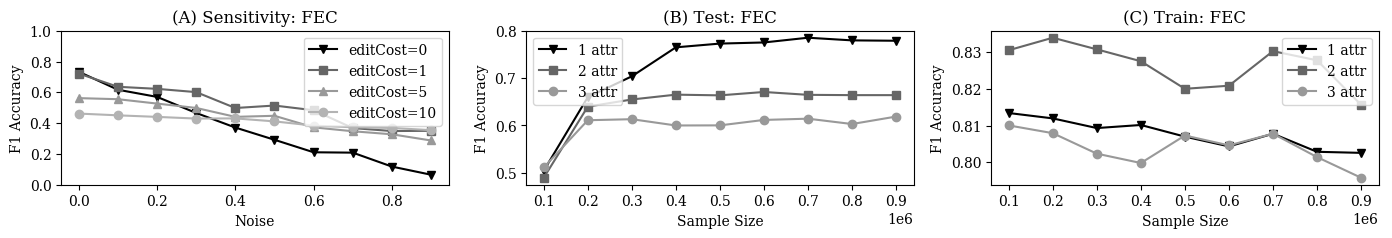
\includegraphics[width=\textwidth]{ac-experiments/exp5.png}
 \caption{\small (A) Regularization by increasing an editCost penalty makes \sys more robust to noisy (mis-specified) quality functions, (B-C) overly expressive transformation templates can lead to overfitting (2 attr) or an infeasibly large search space (3 attr).  
 \label{fig:sensitivity}}
\end{figure*}

 \begin{figure*}[t]
\centering
 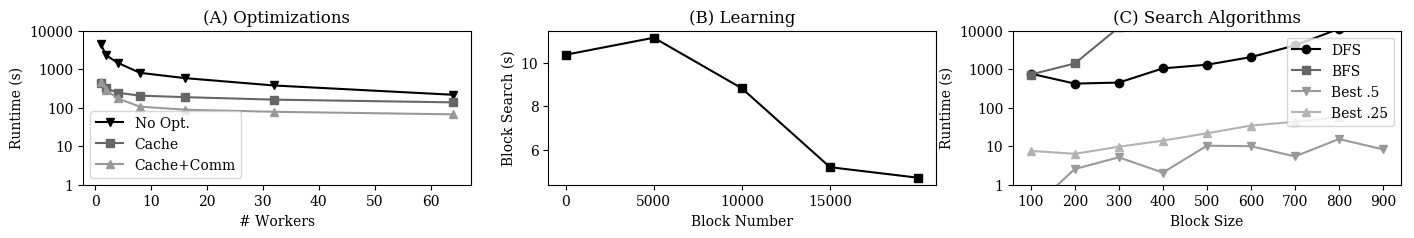
\includegraphics[width=\textwidth]{ac-experiments/exp6.png}
 \caption{\small 
   (A) Both the materialization (Cache) and distributed communication (Comm) optimizations contribute to improved scale-out runtimes.
   (B) The learned pruning rules improve the search costs for each subsequent block-wise partition.  
   (C) Best-first search is better than BFS and DFS; reducing $\gamma$ prunes more candidates at the expense of lower accuracy.  
 \label{fig:opt}}
\end{figure*}


\subsubsection{\sys In Depth}
This subsection uses the FEC setup to study the parameters that affect \sys's accuracy and runtime, the robustness of its cleaning programs, and its algorithmic properties.

\subsubsection{Algorithmic Sensitivity}

\stitle{Block-wise Cleaning} Partitioning the dataset into smaller blocks effectively reduces the problem complexity.  This can have tremendous performance benefits when each block exhibits very few errors that are independent of the other blocks.  \Cref{fig:microbenchmarks}a shows the performance benefits when varying the block size; we define the blocks by partitioning on three different attributes that have different domain sizes.  Reducing the block size directly improves the runtime; the search is effectively non-terminating when blocking is not used.    

\stitle{Language} \Cref{fig:microbenchmarks}b fixes the input to a single block, and evaluates the runtime based on the size of the language $|\Sigma|$.  Increasing the transformations increases the branching factor of the search problem. The search time is exponential in the language, however \sys's learning optimization can identify a pruning model that reduces the runtime to linear.

\stitle{Coupling in the Quality Function} The complexity of the quality function directly affects search time.  A cell-separable quality function is the simplest to optimize because each cell in the relation can be analyzed and cleaned in isolation.  In contrast, a quality function that couples multiple records together is more challenging to optimize because a longer sequence of transformation may be needed to sufficiently clean the records and improve the quality function.  

We evaluate this by artificially coupling between 1-10 records together, and creating a quality function that only improves when an attribute of the coupled records all have the same value.  We perform this coupling in two ways: {\it Random} couples randomly selected records, whereas {\it Correlated} first sorts the relation an attribute and couple records within a continuous range.  We expect that the random coupling requires individual cleaning operations for each record based on their IDs, whereas the correlated setting both allows \sys to exploit the correlated structure to learn effective pruning rules and to clean the coupled records using a single cleaning operation.  \Cref{fig:microbenchmarks}c shows that this is indeed the case when running \sys on a single fixed-size block. {\it Random} slows down exponentially with increased coupling, whereas {\it Correlated} increases linearly.

% The nature of the quality function also affects the search time. Quality functions that couple multiple records together are harder to optimize (Figure \ref{fig:microbenchmarks}c).
% Consider a function that requires that two different records must have the same attribute values.
% More transformations have to be achieved in a particular sequence before an improvement in quality is observed. 
% We selected between 1-10 records at random in each block and created a quality function that coupled these records together.
% As the degree of coupling increases, the search time grows quite drastically.
% We repeated the same experiment where now coupling is correlated with the data, i.e., we sort one of the attributes and couple ``nearby'' records.
% \sys performs significantly better on this version of the task.
% This is due to the learned pruning in \sys.
% Sorting the attributes introduces a systematic correlation in the quality function.
% \sys quickly learns a model which learns this correlation and uses that to prune the search space.

\stitle{Quality Function Complexity} Finally, we incrementally increase the quality function's complexity and show haw it affects the cleaning accuracy.  We add the following constraints in sequence: one functional dependency (FD), a second FD, an entity resolution similarity rule, and a third FD.  We define the quality function as the sum of each constraint's quality function.   \Cref{fig:microbenchmarks}d shows that the F1 accuracy decreases as more constraints are added, however the F1 score is still above $75\%$.  




\subsubsection{Cleaning Generalization and Overfitting}\label{s:expoverfit}
An important characteristic of generating cleaning solutions as {\it programs} is that we can evaluate the program's robustness in terms of machine learning concepts such as overfitting and generalization.    To this end, we examine two concepts in the context of data cleaning: regularizaton and overfitting.  We also find that \sys's high level interface is helpful for iteratively tuning the cleaning process.

\stitle{Regularization}  Misspecified quality functions can cause \sys to output poorly performing cleaning programs.  We simulate this by adding random noise to the output of the quality function. \Cref{fig:sensitivity}A plots the F1-score of \sys on the FEC experiment while varying the amount of noise.  As expected, the output program's F1-score rapidly degrades as the noise increases.  

Machine learning uses regularizing penalty terms to prevent overfitting.  We can similarly add a penalty to the quality function to prevent too many edits.  Each line line shows the edit cost penalty and shows that although the F1 is lower when there is no noise, \sys is more robust to larger amounts of noise. 

\stitle{Overfitting} In machine learning, over-parameterized models may be susceptible to overfitting.  A similar property is possible if the language $\Sigma$ is overly expressive.  We use a transformation template that finds records matching a parameterized predicate and sets an attribute to another value in its instance domain.   We then vary the language expressiveness by increasing number of attributes in the predicate between 1 and 3.  Finally, we run \sys on a training sample of the dataset (x-axis), and report F1 accuracy on the training and a separate test sample (\Cref{fig:sensitivity}B-C).  Note that overfitting occurs when the training accuracy is significantly higher than test accuracy.

Indeed we find an interesting trade-off.  The 1 attribute predicate performed worst on the training sample but outperformed the alternatives on the test sample.  The 2 attribute predicate was more expressive and overfit to the training data.  Finally, the 3 attribute predicate is overly expressive and computationally difficult to search.  Thus, it did not sufficiently explore the search space to reliably identify high quality cleaning programs. 

\stitle{Discussion} We have shown that data cleaning can overfit, and believe this is a potential issue in {\it any} cleaning procedure. These results highlight the importance of domain experts to judge and constrain the cleaning problem in ways that will likely generalize to future data. Further, it shows the value of a high-level interface that experts can use to express these contraints by iteratively tuning the quality function and cleaning language. 

% and evaluate the training and test        Figure \ref{fig:sensitivity}B-C illustrates another interesting aspect of \sys, namely, a property akin to overfitting in machine learning.
% We parametrized the transformation language with single attribute, double attribute, and triple attribute predicates.
% Then, we applied \sys to sample of data.
% We measured the ``in-sample error'' Figure \ref{fig:sensitivity}C, which is the F1 score with records inside the sample, and the ``out-of-sample'' error which is the F1 score on unseen records.
% The more expressive two attribute predicates are most accurate on the in-sample metric, however, we not as accurate as the single attribute predicates on the out-of-sample metric.
% The three sample predicates were very computationally expensive to search so the results are less reliable.
% This result highlights an important point overly specific rules may not apply to future data, and overly general rules, might introduce unwanted side-effects.


\subsubsection{Scaling}
Next, we present preliminary results illustrating the scaling properties of \sys. 

\vspace{1em}

\stitle{Parallelization Optimizations} The experiments run on a cluster of 4 mx.large EC2 instances, and we treat each worker in a distributed (not shared-memory) fashion.   \Cref{fig:opt}a shows the benefits of the materialization and communication optimizations in \Cref{s:parallel}.  {\it No opt.} simply runs best-first search in parallel without any materialization; workers only synchronize at the end of an iteration by sending their top-$\gamma$ candidate programs to the driver, which prunes and redistributes the candidates in the next iteration.  {\it Cache} extends No opt by locally materializing parent programs, and {\it Cache+Comm} further adds the communication optimizations for distributed parallelization.   

The single threaded No Opt setting runs in $4432$s, and the materialization optimization reduces the runtime by $10\times$ to $432$s.   Scaling out improves all methods: at 64 workers, {\it Cache+Comm} takes 67s while {\it Cache} takes 137s.  Surprisingly, although {\it No Opt} with 64 workers is slower than {\it Cache+Comm} by $10\times$, it scales the best because it only synchronizes at the end of an iteration and only communicates candidate programs and their quality values.  In contrast, the alternative methods may communicate materialized relation instances.  

\stitle{Within-Block Learning} Although we have shown how learning reduce the overall search runtime, we show that learning also improves the search speed for individual blocks.  We run single-threaded \sys and report the time to evaluate each block.  \Cref{fig:opt}b shows the $i^{th}$ block that is processed on the x-axis, and the time to process it on the y-axis.   We see that as more blocks are cleaned, the learned pruning classifier is more effective at pruning implausible candidate programs.  This reduces the per-block search time by up to $75\%$.  

\stitle{Search Algorithm Choice} \Cref{fig:opt}c shows that best-first search out-performs naive depth and breadth first search.  We also report \sys when $\gamma=\{0.5, 0.25\}$.  We see that as the block size increases, DFS and BFS quickly become infeasible, whereas \sys runs orders of magnitude more quickly.  In addition, reducing $\gamma$ improves the runtime, however can come at the cost of reduced accuracy by pruning locally sub-optimal but globally optimal candidate programs.  



\subsubsection{Program Structure}
Finally, we present results describing the structure of the data cleaning programs found with \sys.
It is often the case that the program found by \sys is a concise description of the needed data cleaning operations, that is, the total number of cell edits is much larger than the length of the program.
We consider the FEC dataset, the EEG dataset, and GTD dataset.

Sometimes, the program (FEC and GTD) encodes a significant amount of literal values. This happens in entity matching type problems. For these problems, the program length is relatively large, however, the number of cells modified is even larger (up to 10x more).
For datasets like the EEG dataset, the program is very concise (26x smaller than the number of cells modified).
Numerical thresholds are generalize better than categorical find-and-replace operations.

\begin{table}[ht!]
\centering
\label{my-label}
\begin{tabular}{|l|l|l|}
\hline
    & Program Length & Cells Modified \\ \hline \hline
FEC & 6416           & 78342          \\ \hline
EEG & 6              & 161            \\ \hline
GTD & 1014           & 104992 \\ \hline
\end{tabular}
\end{table}


